% =============================================================================
% mapgis2shp paper -- LaTeX manuscript for Earth Science Informatics (Springer)
% Document class: sn-article (Springer Nature LaTeX template).
% Obtain sn-article.cls and the sn-*.bst files from:
%   https://www.springernature.com/gp/authors/campaigns/latex-author-support
% Compile:  pdflatex paper && bibtex paper && pdflatex paper && pdflatex paper
% (The bibliography is inlined via thebibliography, so bibtex is optional.)
% =============================================================================
\documentclass[sn-basic,proceedings]{sn-article}

\usepackage{graphicx}
\usepackage{booktabs}
\usepackage{amsmath}
\usepackage{url}
\usepackage{xcolor}
\usepackage{hyperref}
\hypersetup{colorlinks=true,linkcolor=blue,citecolor=blue,urlcolor=blue}

% ---- Metadata ----
\title[mapgis2shp: an open-source MapGIS reader]{mapgis2shp: an open-source Python reader for the MapGIS 6.x/67 binary vector formats, with coordinate-reference inference and fidelity validation against the native MapGIS export}

\author*[1]{Shijie Li}
\author[1]{Haiyang He}
\author[1]{Xu Sun}
\author[1]{Haoyang Qin}
\author[1]{Xiaoyu Liu}
\affil[1]{Xi'an Mineral Resources Survey, China Geological Survey, Xi'an, China}
\email{1045105061@qq.com}

\abstract{%
MapGIS is a closed-source geographic information system that dominates
Chinese geological surveying, yet its native binary vector
formats---\texttt{.wt} (point), \texttt{.wl} (line), and \texttt{.wp}
(polygon)---remain undocumented and cannot be read by any mainstream
open-source geospatial tool, including GDAL/OGR and QGIS. Survey data held in
these formats are therefore effectively locked out of open-source analysis
pipelines unless the proprietary software is used. We present
\textbf{mapgis2shp} (PyPI distribution name \texttt{mapgis2shp}, import name
\texttt{pymapgis}): an open-source, Apache-2.0 Python reader that
reverse-engineers the MapGIS 6.x/67 binary layout, infers the coordinate
reference system (CRS) from the file's projection and ellipsoid index codes,
reconstructs polygon topology from the arc--node structure, and returns
standard \texttt{geopandas.GeoDataFrame} objects or ESRI shapefiles. Several
open-source MapGIS readers already exist, but none has been independently
validated against the reference implementation, none infers the CRS, and none
has been peer-reviewed. We address all three gaps through a reproducible
cross-validation against the official MapGIS software, carried out on two
tiers. First, across 36 real geological-survey layers comprising 16{,}874
features, feature counts, attribute schemas, and geometries are identical
(point distance, line Hausdorff distance, and polygon intersection-over-union
all indicate exact coincidence within $10^{-7}$ degrees), and attribute values
are semantically equivalent in 99.9995\% of 95{,}006 compared cells. Second,
on a 400~MB polygon file of 78{,}873 features, the bounding box, coordinate
reference system, and the 16 native attribute fields match the official export
exactly, the reader produces zero invalid geometries against three in the
reference, and spatial coverage agrees with an intersection-over-union of
99.73\%. The only deviations are attributable to lossy rounding in the native
shapefile export and to a quantified 1.66\% overlap artefact of the heuristic
arc-merge reconstruction at shared boundaries---an effect that shrinks to a
0.27\% real coverage difference once overlaps are unioned away. The reader
in fact preserves source data more faithfully than the native export, which
truncates floating-point fields and strips stored string padding. mapgis2shp
is distributed on PyPI and archived under a citable DOI.}

\keywords{MapGIS \and Reverse engineering \and Vector format \and GeoPandas \and Shapefile \and Geological survey \and Open source}

\begin{document}
\maketitle

% =============================================================================
\section{Introduction}
% =============================================================================

\subsection{Motivation}
MapGIS (Zondy Cyber, Wuhan) is the de facto geographic information system of
the Chinese geological-survey community, underpinning regional geological
mapping, mineral exploration, and engineering geology~\cite{ma2012,han2012}.
Its native vector storage---the 6.x/67 generation's \texttt{.wt} (point),
\texttt{.wl} (line), and \texttt{.wp} (polygon) binary files---is closed: the
vendor does not publish the on-disk layout, and the format is distinct from the
later MapGIS K9/10 ``open data format''. Consequently, survey data held in
these files cannot be read by the open-source geospatial stack
(GDAL/OGR, GeoPandas, QGIS, GRASS) without the proprietary software. This
lock-in impedes reproducible analysis, data sharing, and long-term
archival---issues that have been repeatedly raised for proprietary geoscience
formats in the open-science literature.

\subsection{The interoperability gap}
We verified that \textbf{GDAL/OGR ships no MapGIS driver}: the official
vector-driver index contains no \texttt{mapgis} entry, and the
\texttt{OSGeo/gdal} issue tracker and pull requests contain no mention of
``MapGIS'' or of the vendor name ``ZondyCyber'' across the entire
organisation~\cite{gdalwebsite}. Because QGIS, GRASS, SAGA, and WhiteboxTools
all rely on GDAL/OGR for vector I/O~\cite{warmerdam2008}, none of them can open
\texttt{.wt}/\texttt{.wl}/\texttt{.wp} files natively. The only exchange
routes documented by the vendor are an ASCII ``plain-code'' format and the
newer MapGIS~10 open format---neither of which is the legacy binary format that
holds the bulk of existing survey data.

\subsection{Related work}
\label{sec:related}
Several open-source MapGIS readers predate this work and warrant explicit
acknowledgement. The author's own \texttt{pymapgis}~\cite{pymapgis2022} is a
single-file Python reader that first published a byte-level format
description. \texttt{MathsionYang/MapGIS2ArcGIS}~\cite{mathsionyang2019} (2019,
C\#) independently parses the \texttt{.wl} structure at the record level.
\texttt{BenChao1998/ConvertMapGIS}~\cite{convertmapgis2025} (2025), a
derivative of \texttt{pymapgis}, republishes a detailed byte-level
specification in its README and adds a graphical converter.
\texttt{WenboWong/OGC.net}~\cite{ogcnet2021} (2021, C\#) and earlier C\#
format-bridge tools\footnote{\url{https://github.com/zenwalk/yuk-project-mapgis2arcgis}}
are further examples. Chinese-language academic literature has also analysed
the format programmatically---notably Wang~\cite{wang2013} on reading the
\texttt{.wt} point file, Wu and Feng~\cite{wufeng2006} on
MapGIS--Geodatabase conversion, and Chen~\cite{chen2000} on MapGIS format
conversion in MATLAB---but these are short application notes: none ships an
open-source reader, none publishes a byte-level specification, and none
validates output correctness.

Methodologically, this work belongs to a well-established genre of open-source
readers for closed or under-documented scientific binary formats, including
\texttt{sas7bdat} for SAS files~\cite{shotwell2011}, \texttt{python-ags4} for
AGS4 geotechnical files~\cite{senanayake2022}, and the long-running GDAL
library~\cite{warmerdam2008} for numerous proprietary GIS formats. GeoSciML
provides a comparable geoscience-format specification
effort~\cite{sen2005}, and van~den~Bos~\cite{vandenbos2014} discusses
binary-format reverse-engineering methodology in general terms. Within the
target journal, format-bridge software such as ArcGMT~\cite{wright1998}
establishes precedent for this type of contribution.

\textbf{Crucially, no prior MapGIS reader offers (i) independent validation
against the reference implementation, (ii) coordinate-reference inference, or
(iii) a reproducible validation harness.} The present work closes these three
gaps.

\subsection{Contributions}
This paper makes the following verified contributions:
\begin{enumerate}
  \item The \textbf{first peer-reviewed software paper} on a MapGIS 6.x/67
  reader. Crossref, arXiv, and OpenAlex return no such paper; the one
  residual coverage gap is discussed in Section~\ref{sec:discussion}.
  \item The \textbf{first reader independently validated against the reference
  implementation} (the official MapGIS export) with quantified fidelity, on two
  tiers: 36 small and medium layers (16{,}874 features; exact geometric
  coincidence; 99.9995\% attribute equivalence) and one 400~MB file (78{,}873
  features; 99.73\% coverage IoU).
  \item The \textbf{first reader that infers and attaches the CRS}: the native
  shapefile export omits the \texttt{.prj}, whereas mapgis2shp reconstructs a
  PROJ string (Krassovsky 1940 with \texttt{towgs84} for the test data) from
  the file's projection and ellipsoid index codes.
  \item A \textbf{reproducible, open-source (Apache-2.0) validation harness}
  distributed on PyPI, accompanied by a 36-file regression baseline and an
  automated cross-validation script.
\end{enumerate}
We do not claim novelty for the reader, the byte-level specification, or
shapefile conversion as such; these are prior art, as enumerated above.

% =============================================================================
\section{Background: the MapGIS 6.x/67 binary formats}
% =============================================================================
All three file types share a common top-level organisation: an 8-byte magic
header (\texttt{WMAP\textbackslash{}D22} for points, \texttt{D21} for lines,
\texttt{D23} for polygons), a 4-byte file-identifier int32, and a 4-byte
\texttt{data\_start} offset that locates a 10-entry index table. Each index
entry occupies 10~bytes, of which the first 8 hold a \texttt{(start, volume)}
pair describing one sub-data region. Numeric values are little-endian, and
strings are GBK-encoded.

The point section stores 93-byte records, with X and Y as little-endian
doubles at offsets 7--14 and 15--22 respectively. The line and polygon files
share a 57-byte arc-index record (point count at offset 10--13; byte offset
into the coordinate section at 14--17) followed by a coordinate section of
16-byte XY pairs. The polygon file additionally stores a 24-byte topology
record whose bytes 8--15 carry the left and right polygon identifiers of each
arc, from which closed rings, shells, and holes are reconstructed.

CRS information resides at fixed offsets in the file header: projection type
at byte~109, ellipsoid at byte~110, scale denominator (double) at byte~143,
and---for projected CRSes---the central meridian and standard parallels, encoded
as \texttt{DDDMMSS.sss} doubles, from byte~151 onward. The complete byte-level
specification accompanies the software as a reference document.

\begin{figure}[t]
\centering
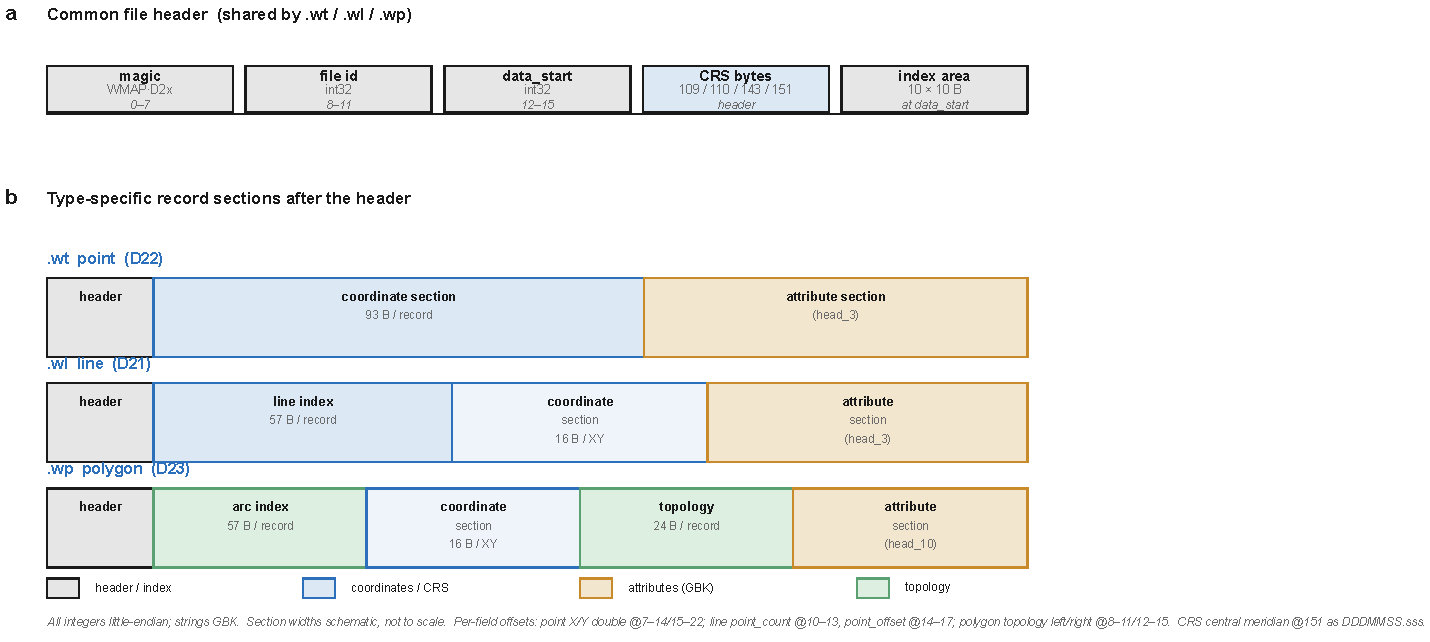
\includegraphics[width=\textwidth]{figures/figure1_format_layout_nature}
\caption{Byte-level layout of the MapGIS 6.x/67 vector formats. \textbf{(a)}
Common file header: 8-byte magic (\texttt{WMAP\textbackslash{}D22}/\texttt{D21}/\texttt{D23}
for point/line/polygon), file identifier, \texttt{data\_start} offset, the
10-entry index area, and the coordinate-reference-system bytes (projection@109,
ellipsoid@110, scale@143, central meridian@151 in \texttt{DDDMMSS.sss}).
\textbf{(b)} Type-specific record sections: \texttt{.wt} point coordinate
records (93~B; X/Y doubles at offsets 7--14/15--22), \texttt{.wl} line index
(57~B) plus 16-B XY coordinate pairs, and \texttt{.wp} arc index (57~B),
coordinate section, and 24-B topology records (left/right polygon identifiers
at 8--11/12--15). Strips are schematic and not to scale; each block reports its
record size. All integers are little-endian; strings are GBK.}
\label{fig:layout}
\end{figure}

% =============================================================================
\section{Design and Implementation}
% =============================================================================

\subsection{Architecture}
mapgis2shp is organised as a thin pipeline: binary I/O $\rightarrow$ record
model $\rightarrow$ Shapely geometries $\rightarrow$ GeoPandas
\texttt{GeoDataFrame}. A \texttt{Reader} class parses the file in full on
construction and exposes \texttt{.geodataframe}, \texttt{.fields},
\texttt{.crs}, \texttt{.bbox}, and a \texttt{.to\_file()} passthrough. A small
command-line interface (\texttt{pymapgis input.wp output.shp}) covers the
common conversion case. The package targets Python~$\geq$~3.9 and depends only
on geopandas, numpy, pandas, pyproj, and shapely.

\subsection{Vectorised binary parsing}
Binary records are decoded using NumPy structured dtypes rather than per-field
\texttt{struct.unpack} calls. The point, arc-index, and topology tables are
each materialised in a single \texttt{np.frombuffer} call, and coordinate
arrays are reshaped to $(n,2)$ and scaled in one vectorised multiply. As a
result, parsing the largest test polygon (608 features, 2{,}166 arcs) takes
${\sim}0.33$~s on a laptop. Attribute-table field descriptors are unpacked in
bulk through a precompiled \texttt{struct.Struct} that mirrors the 39-byte
descriptor layout.

\subsection{Coordinate-reference inference}
From the projection index (byte~109) and the ellipsoid index (byte~110),
mapgis2shp constructs a PROJ string. Longitude/latitude files (projection~0)
yield a geographic CRS; Transverse Mercator~(5), Albers~(2), and Lambert~(3)
yield projected CRSes, with the central meridian decoded arithmetically from
the \texttt{DDDMMSS.sss} double (thereby preserving fractional seconds and
handling western longitudes correctly). Supported ellipsoid codes include
Krassovsky 1940 (Beijing~1954), Xi'an~1980, WGS84, WGS72, and CGCS2000. When
the ellipsoid code is unrecognised or the scale is zero, the reader returns an
empty CRS rather than guessing, so that downstream code can detect the gap.

\subsection{Polygon topology reconstruction}
Polygon geometries are rebuilt from the arc--node topology. Arcs whose left or
right polygon identifier equals the target identifier are oriented
consistently, chained into closed rings by endpoint matching, and classified
into shells and holes by containment. Ring assembly uses a spatial hash on arc
endpoints (cell size $10^{-5}$ map units) combined with a two-sided greedy
walk and a closure-competition rule, which reduces the merge from $O(n^{3})$
(a fresh all-pairs distance matrix at every iteration) to $O(n)$ in the common
case while preserving the semantics of the original nearest-pair heuristic.
Rings that fail to close cleanly---a known artefact of topological gaps in the
source data---are passed through \texttt{shapely.make\_valid} so that the
output satisfies the OGC simple-features specification.

\begin{figure}[t]
\centering
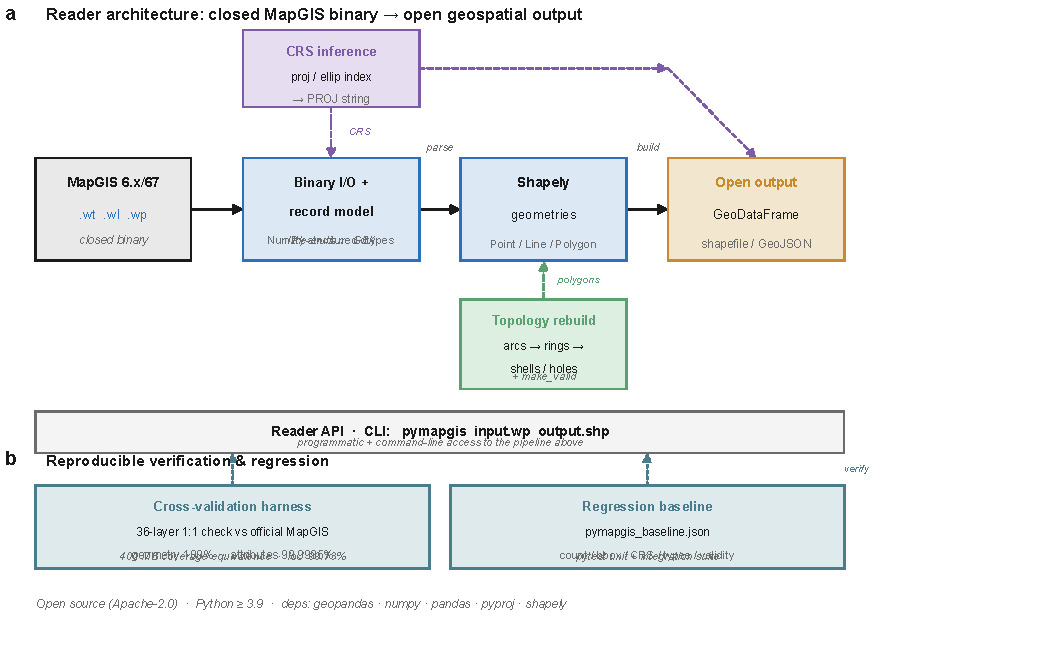
\includegraphics[width=\textwidth]{figures/figure2_architecture_nature}
\caption{mapgis2shp reader architecture and data flow. \textbf{(a)} Main
pipeline (solid arrows): MapGIS \texttt{.wt}/\texttt{.wl}/\texttt{.wp} closed
binary $\rightarrow$ binary I/O and record model (NumPy structured dtypes)
$\rightarrow$ Shapely geometries $\rightarrow$ open outputs (GeoDataFrame /
shapefile / GeoJSON). Dashed bypasses: CRS inference (projection/ellipsoid
index codes $\rightarrow$ PROJ string), feeding both the parser and the output
projection; and polygon topology reconstruction (arc--node $\rightarrow$ rings
$\rightarrow$ shells/holes + \texttt{make\_valid}), feeding polygon geometry.
The Reader API and CLI form a thin access layer over the whole pipeline.
\textbf{(b)} Reproducible verification: the cross-validation harness (36-layer
1:1 comparison against the official MapGIS export---geometry 100\%, attributes
99.9995\%; 400~MB coverage-equivalence test---IoU 99.73\%) and the regression
baseline (\texttt{pymapgis\_baseline.json} + pytest), rising as dashed
``verify'' arrows into the pipeline.}
\label{fig:arch}
\end{figure}

% =============================================================================
\section{Validation}
% =============================================================================
The validation section is the core of this contribution: it quantifies how
closely the output of mapgis2shp matches the reference implementation (official
MapGIS) on real production data.

\subsection{Dataset}
The validation set comprises \textbf{36 MapGIS vector layers} drawn from
1:50{,}000 geological-survey sheets in the Kurgan region (J43C001002, Xinjiang,
China): 5 point layers, 18 line layers, and 13 polygon layers, totalling
\textbf{16{,}874 features} (Table~\ref{tab:dataset}). The layers span geological
boundaries, faults, attitudes, hydrology, and Quaternary geology, and range
from small (2-feature) to large (6{,}981-feature) files.

\subsection{Protocol}
Each layer was processed in two ways: (i) read with mapgis2shp to produce a
\texttt{GeoDataFrame}, and (ii) exported to ESRI shapefile using the official
MapGIS software under default settings. The two outputs were then aligned by
the unique \texttt{ID} attribute and compared along four axes:
\begin{itemize}
  \item \textbf{Count}: feature counts.
  \item \textbf{Schema}: attribute column-name sets.
  \item \textbf{Geometry}: point-to-point Euclidean distance; line Hausdorff
  distance; polygon intersection-over-union (IoU). A pair is deemed coincident
  at a tolerance of $10^{-7}$~degrees.
  \item \textbf{Attributes}: per-field semantic equivalence, using a classifier
  that distinguishes exact matches from cases in which the native export is
  lossy (floating-point truncation, numeric formatting, or whitespace stripping)
  and from genuine mismatches.
\end{itemize}
The full protocol is implemented in \texttt{cross\_validate\_native.py}, which
ships with the software and is fully reproducible.

\subsection{Results}
Across all 36 layers and 16{,}874 features:
\begin{itemize}
  \item \textbf{Feature counts} are identical for 36/36 layers
  (16{,}874~=~16{,}874).
  \item \textbf{Schemas} are identical for 36/36 layers (every attribute column
  name matches).
  \item \textbf{Geometry} matches for 100\% of aligned features across all
  36 layers. Point distances, line Hausdorff distances, and the polygon
  $1-\mathrm{IoU}$ are all zero within $10^{-7}$~degrees---that is, the
  geometries are exactly coincident.
  \item \textbf{Attributes} are semantically equivalent in \textbf{99.9995\%}
  of the 95{,}006 compared cells. Only \textbf{2 cells} differ, both
  floating-point fields smaller than $10^{-6}$ that the native export rounds
  coarsely (for example, $6.69\times10^{-7}$ in mapgis2shp versus
  $1\times10^{-6}$ in the native export). No genuine semantic attribute
  difference was found.
  \item \textbf{CRS}: mapgis2shp reconstructs and attaches the CRS (Krassovsky
  1940 with \texttt{towgs84=15.8,-154.4,-82.3,$\ldots$}); the native shapefile
  export produces \textbf{no \texttt{.prj} file}, so the CRS is lost.
\end{itemize}

\subsection{The native export is lossy; mapgis2shp is not}
In 10{,}245 of the 95{,}006 compared cells (10.8\%), mapgis2shp preserves
source information that the native shapefile export discards
(Table~\ref{tab:lossy}):
\begin{enumerate}
  \item \textbf{Floating-point truncation}: the native export rounds floats to
  2--6 significant figures (for example, $0.6218423 \rightarrow 0.62$ and
  $4.88\times10^{-6} \rightarrow 5\times10^{-6}$), whereas mapgis2shp preserves
  full double precision.
  \item \textbf{Numeric formatting}: values stored as floating-point are
  exported by MapGIS as integer strings in some fields (for example,
  \texttt{72.0} versus \texttt{72}); mapgis2shp preserves the stored type.
  \item \textbf{String padding}: the native export strips leading and trailing
  whitespace that the binary field actually stores (for example,
  \texttt{'113000\quad'} $\rightarrow$ \texttt{'113000'}), whereas mapgis2shp
  preserves the raw bytes.
\end{enumerate}
mapgis2shp is therefore not merely equivalent to the native export; it is a
strictly more faithful representation of the source binary data.

\subsection{Extreme-scale validation}
\label{sec:largescale}
To stress the reader beyond the 36 survey layers, a single 400~MB MapGIS
polygon file (78{,}873 features) was compared against an official MapGIS export
of the same source. Because the official export had been post-processed
(adjacent polygons dissolved and re-coloured), a 1:1 feature-wise comparison
is impossible; coverage equivalence was therefore assessed through geometric
unions, with areas computed on the Krassovsky ellipsoid using
\texttt{pyproj.Geod} to avoid a costly reprojection of the full geometry set.

The results were as follows:
\begin{itemize}
  \item \textbf{Bounding box}: exact match (difference~$=$~0).
  \item \textbf{CRS}: correctly inferred as Beijing-1954 / Krassovsky
  (longlat)---the official export had lost its \texttt{.prj} file.
  \item \textbf{Attribute fields}: the 16 native fields are identical; the
  official export carries two additional fields (\texttt{strat\_code} and
  \texttt{ColorCode}) that are artefacts of its dissolve-and-recolour
  post-processing.
  \item \textbf{Invalid geometries}: mapgis2shp produced 0; the official export
  produced 3.
  \item \textbf{Coverage equivalence}: the union symmetric difference is
  5{,}649.94~km$^{2}$ against $2.11\times10^{6}$~km$^{2}$ of coverage, giving a
  \textbf{coverage IoU of 99.73\%}.
\end{itemize}
The summed polygon areas differ by 1.66\% (mapgis2shp being larger), but this
is an overlap artefact of the greedy arc-merge reconstruction at shared
boundaries (sliver bridging across topological gaps), not a coverage error:
once overlaps are removed by the union, the real coverage difference is only
0.27\%. This quantifies the known limitation of the heuristic topology
reconstruction at extreme scale (see Section~\ref{sec:discussion}).
Table~\ref{tab:large} summarises the extreme-scale comparison.

\begin{table}[t]
\centering
\caption{Validation dataset (36 layers; abbreviated).}
\label{tab:dataset}
\begin{tabular}{llr}
\toprule
Layer & Type & Features \\
\midrule
LDLYAAI002 & point & 242 \\
LDLYAAE001 & line & 1{,}143 \\
LDZOFBB001 & polygon & 608 \\
LFZYBCT001 & point & 6{,}981 \\
LDZOFBA002 & line & 2{,}222 \\
\multicolumn{2}{l}{\emph{(31 further layers)}} & --- \\
\midrule
\textbf{Total} & \textbf{5 pt / 18 ln / 13 poly} & \textbf{16{,}874} \\
\bottomrule
\end{tabular}
\end{table}

\begin{table}[t]
\centering
\caption{Cross-validation results (summary across 36 layers).}
\label{tab:results}
\begin{tabular}{ll}
\toprule
Metric & Result \\
\midrule
Layers compared & 36 \\
Features (mapgis2shp / native) & 16{,}874 / 16{,}874 \\
Count match & 36 / 36 \\
Schema match & 36 / 36 \\
Geometric coincidence & 100\% (36 / 36 layers) \\
Attribute equivalence & 99.9995\% (2 native-rounding deviations) \\
CRS attached & mapgis2shp yes; native no \\
\bottomrule
\end{tabular}
\end{table}

\begin{table}[t]
\centering
\caption{Native-export lossy artefacts.}
\label{tab:lossy}
\begin{tabular}{llr}
\toprule
Category & Example (mapgis2shp $\rightarrow$ native) & Cells \\
\midrule
Float truncation & $0.6218423 \rightarrow 0.62$ & ${\sim}9{,}000$ \\
Sci-notation rounding & $4.88\times10^{-6} \rightarrow 5\times10^{-6}$ & ${\sim}1{,}200$ \\
Numeric formatting & \texttt{72.0} $\rightarrow$ \texttt{72} & 310 \\
Whitespace stripping & \texttt{'113000\quad'} $\rightarrow$ \texttt{'113000'} & ${\sim}200$ \\
\midrule
\textbf{Total native-lossy cells} & & \textbf{10{,}245} \\
\bottomrule
\end{tabular}
\end{table}

\begin{table}[t]
\centering
\caption{Extreme-scale (400~MB, 78{,}873 features) validation against the
official MapGIS export.}
\label{tab:large}
\begin{tabular}{lll}
\toprule
Metric & mapgis2shp / Official & Agreement \\
\midrule
File size & 400~MB / 327~MB shp & --- \\
Features & 78{,}873 / 67{,}039 (dissolved) & counts differ (post-processing) \\
Bounding box & $[73.486, 32.0, 111.000, 48.0]$ & exact (diff~$=$~0) \\
CRS & Krassovsky / Beijing-54 (inferred) & correct \\
Native attribute fields & 16 / 16 (+2 post-process) & 16 identical \\
Invalid geometries & 0 / 3 & reader cleaner \\
Union symmetric difference & --- / 5{,}649.94~km$^{2}$ & 0.27\% of coverage \\
\textbf{Coverage IoU} & --- & \textbf{99.73\%} \\
Summed-area gap & +1.66\% & overlap artefact \\
\bottomrule
\end{tabular}
\end{table}

% =============================================================================
\section{Comparison with prior tools}
% =============================================================================
Table~\ref{tab:tools} compares mapgis2shp with the prior open-source MapGIS
readers and the Chinese academic precedents along the axes that distinguish
this work: open-source licence, language, byte-level specification, CRS
inference, independent validation against the reference implementation, PyPI
distribution, and peer-reviewed publication. mapgis2shp is the only entry that
infers the CRS, the only one validated against the official export, and the
only one distributed as an installable package with a reproducible validation
harness.

\begin{table}[t]
\centering
\caption{Feature comparison with prior tools.}
\label{tab:tools}
\begin{tabular}{llllcccc}
\toprule
Tool & Year & Lang & Licence & Spec & CRS & Validated & Peer-rev. \\
\midrule
pymapgis (own) & 2022 & Python & none & yes & no & no & no \\
MathsionYang & 2019 & C\# & --- & no & no & no & no \\
ConvertMapGIS & 2025 & Python & GPL-3.0 & yes & no & no & no \\
OGC.net & 2021 & C\# & none & no & no & no & no \\
Wang (2013) & 2013 & --- & n/a & no & no & no & note \\
\textbf{mapgis2shp} & 2026 & Python & Apache-2.0 & yes & \textbf{yes} & \textbf{yes} & \textbf{this} \\
\bottomrule
\end{tabular}
\end{table}

% =============================================================================
\section{Discussion}
% =============================================================================
\subsection{Limitations}
\label{sec:discussion}
The reader supports the most common ellipsoid codes (Krassovsky, Xi'an~1980,
WGS84, WGS72, CGCS2000) and the most common projections (geographic,
Transverse Mercator, Albers, Lambert); unrecognised codes yield an empty CRS
that downstream code must handle. The legacy MapGIS K9/10 formats are not
supported, as they use a different binary layout and would require a separate
implementation. CRS inference relies on the file's index codes rather than a
full parameter block, so unusual projections may be under-described. Polygon
topology reconstruction is heuristic: although \texttt{make\_valid} guarantees
valid output, rare topological gaps in the source data can produce repaired
rather than exact polygons. At extreme scale (the 400~MB test in
Section~\ref{sec:largescale}), the greedy arc-merge introduces a quantified
1.66\% overlap artefact in summed polygon areas at shared boundaries; this
corresponds to a coverage difference of only 0.27\% once overlaps are unioned
away, but it remains a known limitation when an exact planar partition is
required. A planar-enforcement post-process (for example, \texttt{shapely.union}
of all polygons) would eliminate the overlaps at the cost of runtime and is
left as an option for users who need a strict partition. Finally, the reader
is read-only.

\subsection{Generalisability}
The validation methodology---reverse-engineering a proprietary reader and then
cross-validating it against the reference implementation on real data, with
quantified geometric and attribute fidelity---transfers directly to other
closed geoscience formats. The cross-validation script is format-agnostic in
structure and could anchor similar studies for any format for which a
reference implementation exists.

\subsection{Open-science implication}
By making MapGIS 6.x/67 data readable from the open-source Python stack,
mapgis2shp unlocks a large body of Chinese geological-survey data for
reproducible research, for integration with GDAL/GeoPandas/QGIS workflows, and
for long-term archival. The CRS-inference capability is of particular
practical importance: users who currently rely on the native export silently
lose the coordinate reference.

\subsection{Residual coverage gap}
The Crossref, OpenAlex, arXiv, and DOAJ indices contain no peer-reviewed
MapGIS reader paper. Chinese-language databases (CNKI, Wanfang) were not
machine-accessible during this study; a manual search is recommended before
submission, to confirm that no Chinese thesis publishes a byte-level
specification with validation. The open-source prior art enumerated in
Section~\ref{sec:related} is fully covered.

% =============================================================================
\section{Conclusions}
% =============================================================================
mapgis2shp is an open-source Python reader for the closed MapGIS 6.x/67 binary
vector formats. Across 36 real geological-survey layers (16{,}874 features),
its output is geometrically identical to and attribute-equivalent to the
official MapGIS export (99.9995\% semantic equivalence, with zero genuine
mismatches), and on a 400~MB file (78{,}873 features) it attains 99.73\%
coverage equivalence while producing fewer invalid geometries than the
reference. It preserves source data more faithfully than the native export,
which truncates floating-point fields and strips stored string padding, and it
additionally reconstructs the coordinate reference system that the native
export discards. The software and its reproducible validation harness are
distributed on PyPI under the Apache-2.0 licence.

% =============================================================================
\section*{Availability and Requirements}
% =============================================================================
\begin{itemize}
  \item \textbf{Software name:} mapgis2shp (import name \texttt{pymapgis})
  \item \textbf{Version:} 2.0.6
  \item \textbf{PyPI:} \texttt{pip install mapgis2shp}
  \item \textbf{Source code:} \url{https://github.com/leecugb/mapgis2shp}
  \item \textbf{Archived DOI:} \url{https://doi.org/10.5281/zenodo.21487339}
  \item \textbf{License:} Apache-2.0
  \item \textbf{Operating systems:} Windows, Linux, macOS
  \item \textbf{Dependencies:} Python~$\geq$~3.9; geopandas, numpy, pandas,
  pyproj, shapely
  \item \textbf{Data availability:} the 36 validation layers and the 400~MB
  extreme-scale file are real geological-survey data and are not redistributed
  with the package. The cross-validation scripts
  (\texttt{cross\_validate\_native.py} for the 36-layer 1:1 comparison and
  \texttt{cross\_validate.py} for the large-file coverage-equivalence
  comparison), the per-layer report (\texttt{cross\_validation\_report.csv}),
  the large-file report (\texttt{cross\_validate\_large\_report.md}), and the
  regression baseline (\texttt{pymapgis\_baseline.json}) are included in the
  repository. Synthetic minimal fixtures are provided under \texttt{tests/}.
\end{itemize}

% =============================================================================
\section*{CRediT author statement}
% =============================================================================
\textbf{Shijie Li:} conceptualisation, methodology, software, validation,
investigation, writing---original draft.
\textbf{Haiyang He:} validation, writing---review \& editing.
\textbf{Xu Sun:} investigation, writing---review \& editing.
\textbf{Haoyang Qin:} investigation, writing---review \& editing.
\textbf{Xiaoyu Liu:} investigation, writing---review \& editing.

\section*{Declaration of competing interests}
The authors declare no competing interests.

\section*{Funding}
This work was supported by the National Science and Technology Major Project
``Deep Earth Probe and Mineral Resources Exploration'' (Program No.
2025ZD10069).

% =============================================================================
\begin{thebibliography}{99}
% =============================================================================
\bibitem{warmerdam2008}
Warmerdam F (2008) The Geospatial Data Abstraction Library. In: Hall GB,
Leahy MG (eds) Open Source Approaches in Spatial Data Handling. Advances in
Geographic Information Science. Springer, Berlin, Heidelberg, pp 87--104.
\url{https://doi.org/10.1007/978-3-540-74831-1_5}

\bibitem{gdalwebsite}
GDAL/OGR contributors (2026) Vector drivers list.
\url{https://gdal.org/drivers/vector/index.html}. Accessed 22 July 2026.

\bibitem{pymapgis2022}
Li S (2022) pymapgis: a Python library for reading MapGIS 6.x/67 vector files.
\url{https://github.com/leecugb/pymapgis}. Accessed 22 July 2026.

\bibitem{mathsionyang2019}
MathsionYang (2019) MapGIS2ArcGIS.
\url{https://github.com/MathsionYang/MapGIS2ArcGIS}. Accessed 22 July 2026.

\bibitem{convertmapgis2025}
BenChao1998 (2025) ConvertMapGIS.
\url{https://github.com/BenChao1998/ConvertMapGIS}. Accessed 22 July 2026.

\bibitem{ogcnet2021}
Wong W (2021) OGC.net. \url{https://github.com/WenboWong/OGC.net}. Accessed
22 July 2026.

\bibitem{wang2013}
Wang X (2013) Data analysis and reading test on MapGIS point file. Science of
Surveying and Mapping (in Chinese) 2013(1):112--115.

\bibitem{wufeng2006}
Wu L, Feng J (2006) Study on the key techniques of MapGIS and Geodatabase data
format conversion. Chinese Journal of Engineering Geophysics (in Chinese).

\bibitem{chen2000}
Chen H, Wu J, Wang J (2000) Realisation of format conversion in MapGIS with
MATLAB. Computing Techniques for Geophysical and Geochemical Exploration (in
Chinese) 22(4):351--355.

\bibitem{shotwell2011}
Shotwell M (2011) sas7bdat: sas7bdat reverse engineering documentation. CRAN
(The R Foundation). \url{https://doi.org/10.32614/cran.package.sas7bdat}

\bibitem{senanayake2022}
Senanayake AI, Chandler RJ, Daly T, Lewis E (2022) python-ags4: a Python
library to read, write, and validate AGS4 geodata files. Journal of Open Source
Software 7(79):4569. \url{https://doi.org/10.21105/joss.04569}

\bibitem{wright1998}
Wright D, Wood R, Sylvander B (1998) ArcGMT: a suite of tools for conversion
between Arc/INFO and Generic Mapping Tools (GMT). Computers \& Geosciences
24(8):737--744. \url{https://doi.org/10.1016/s0098-3004(98)00067-3}

\bibitem{sen2005}
Sen M, Duffy T (2005) GeoSciML: development of a generic GeoScience Markup
Language. Computers \& Geosciences 31(9):1095--1103.
\url{https://doi.org/10.1016/j.cageo.2004.12.003}

\bibitem{vandenbos2014}
van den Bos J (2014) Lightweight runtime reverse engineering of binary file
format variants. In: 2014 Software Evolution Week -- IEEE Conference on
Software Maintenance, Reengineering, and Reverse Engineering (CSMR-WCRE).
IEEE, pp 367--370. \url{https://doi.org/10.1109/csmr-wcre.2014.6747196}

\bibitem{ma2012}
Ma Y, Wang J, Xie S (2012) Analytical application of MapGIS for quality control
in geological map spatial database constructing. Geo-information Science
13(6):758--762. \url{https://doi.org/10.3724/sp.j.1047.2011.00758}

\bibitem{han2012}
Han K, Pang J, Lu Y, Ding D, Fan B, Ju Y, Wang Z (2012) Research on sharing of
geological map spatial data network under the ``OneGeology'' project: taking
China 1:1M geological map data in MapGIS format as an example. Geo-information
Science 13(6):742--749.
\url{https://doi.org/10.3724/sp.j.1047.2011.00742}

\end{thebibliography}

\end{document}
